%%%%%%%%%%%%%%%%%%%%%%%%%%%%%%%%%%%%%%%%%%%%%%%%
%% Compile the master file!
%% 		Slides: Antonio Machicao y Priemer
%% 		Course: GK Linguistik
%%%%%%%%%%%%%%%%%%%%%%%%%%%%%%%%%%%%%%%%%%%%%%%%


%%%%%%%%%%%%%%%%%%%%%%%%%%%%%%%%%%%%%%%%%%%%%%%%%%%%
%%%             Metadata                         
%%%%%%%%%%%%%%%%%%%%%%%%%%%%%%%%%%%%%%%%%%%%%%%%%%%%      

\title{Grundkurs Linguistik}

\subtitle{Sprache \& Sprachwissenschaft II}

\author[A. Machicao y Priemer]{
	{\small Antonio Machicao y Priemer}
	\\
	{\footnotesize \url{http://www.linguistik.hu-berlin.de/staff/amyp}}
	%	\\
	%	\href{mailto:mapriema@hu-berlin.de}{mapriema@hu-berlin.de}}
}

\institute{Institut für deutsche Sprache und Linguistik}

\date{ }

%\publishers{\textbf{6. linguistischer Methodenworkshop \\ Humboldt-Universität zu Berlin}}

%\hyphenation{nobreak}


%%%%%%%%%%%%%%%%%%%%%%%%%%%%%%%%%%%%%%%%%%%%%%%%%%%%
%%%             Preamble's End                   
%%%%%%%%%%%%%%%%%%%%%%%%%%%%%%%%%%%%%%%%%%%%%%%%%%%%       


%%%%%%%%%%%%%%%%%%%%%%%%%      
\huberlintitlepage

\iftoggle{toc}{
\frame{
\begin{multicols}{2}
	\frametitle{Inhaltsverzeichnis}
	\tableofcontents
	%[pausesections]
\end{multicols}
	}
	}

%%%%%%%%%%%%%%%%%%%%%%%%%%%%%%%%%%
%%%%%%%%%%%%%%%%%%%%%%%%%%%%%%%%%%
%%%%%LITERATURE:

%% Allgemein
\nocite{Glueck&Roedel16a}
\nocite{Schierholz&Co18}
\nocite{Luedeling2009a}
\nocite{Meibauer&Co07a} 
\nocite{Repp&Co15a} 

%% Sprache & Sprachwissenschaft
\nocite{Fries16c} %Adäquatheit
\nocite{Fries16a} %Grammatikalität
\nocite{Fries&MyP16c} %GG
\nocite{Fries&MyP16b} %Akzeptabilität
\nocite{Fries&MyP16d} %Kompetenz vs. Performanz
\nocite{MuellerGT-Eng2} %Grammatical Theory (2nd Ed.)


%%%%%%%%%%%%%%%%%%%%%%%%%%%%%%%%%%%
%%%%%%%%%%%%%%%%%%%%%%%%%%%%%%%%%%%
\section{Sprache \& Sprachwissenschaft II}

%%%%%%%%%%%%%%%%%%%%%%%%%%%%%%%%%%%
	
	
%%%%%%%%%%%%%%%%%%%%%%%%%%%%%%%%%%%
%%%%%%%%%%%%%%%%%%%%%%%%%%%%%%%%%%%
\subsection{Grammatik}
%% MyP: Contents
\iftoggle{sectoc}{
\frame{
%\begin{multicols}{2}
\frametitle{~}
	\tableofcontents[currentsubsection, subsubsectionstyle=hide]
%\end{multicols}
}
}

%% StM: Contents
\iftoggle{gliederung}{
	
	\outline{
		\begin{itemize}
			
			\item \blaubf{Grammatik}
			\item Grammatikbegriff
			\item Modularität der Grammatik
			%% Lexikon
			%% Phonologische Komponente
			%% Morphologische Komponente
			%% Syntaktische Komponente
			%% Semantische Komponente
			%% Architektur des Sprachsystems
			\item Linguistische Teildisziplinen
			\item Linguistik als Geistes- und/oder Naturwissenschaft
			\item Sprachwissenschaft \vs Linguistik
			
		\end{itemize}
	}
}
%%%%%%%%%%%%%%%%%%%%%%%%%%%%%%%%%%%
	
\begin{frame}{Grammatik}
	\begin{itemize}
		\item Komplexität des Sprachsystems (Einheiten + Regeln) ist den Sprechern meist \textbf{nicht bewusst}.
		\item[]
		\item Die Linguistik interessiert sich für das unbewusste, internalisierte System, d.h.\ für die sprachliche \textbf{Kompetenz} der Sprecher.
		\item[]
		\item Diese Kompetenz bildet die Grammatik einer Sprache.
	\end{itemize}
	
	\begin{block}<2->{Grammatik}
		System, das Laute/""Lautkombinationen und Bedeutungen \textbf{regelhaft einander zuordnet} und das gesamte Regelsystem einer Sprache umfasst.
	\end{block}	
\end{frame}


%%%%%%%%%%%%%%%%%%%%%%%%%%%%%%%%%%%
%%%%%%%%%%%%%%%%%%%%%%%%%%%%%%%%%%%
\subsection{Grammatikbegriff}

%% MyP: Contents
\iftoggle{sectoc}{
\frame{
%\begin{multicols}{2}
\frametitle{~}
	\tableofcontents[currentsubsection, subsubsectionstyle=hide]
%\end{multicols}
}
}

%% StM: Contents
\iftoggle{gliederung}{
	
	\outline{
		\begin{itemize}
			
			\item Grammatik
			\item \blaubf{Grammatikbegriff}
			\item Modularität der Grammatik
			%% Lexikon
			%% Phonologische Komponente
			%% Morphologische Komponente
			%% Syntaktische Komponente
			%% Semantische Komponente
			%% Architektur des Sprachsystems
			\item Linguistische Teildisziplinen
			\item Linguistik als Geistes- und/oder Naturwissenschaft
			\item Sprachwissenschaft \vs Linguistik
			
		\end{itemize}
	}
}
%%%%%%%%%%%%%%%%%%%%%%%%%%%%%%%%%%%

\begin{frame}{Grammatikbegriff}

\begin{itemize}
	\item<1-> Grammatik im engeren Sinne als \textbf{Lehre} von \textbf{morphologischen} und \textbf{syntaktischen} Regularitäten einer Sprache. Unter dieser Auffassung bleiben die Phonologie und die Semantik als Teilbereiche der Sprachwissenschaft ausgeklammert (\textbf{traditionelle Definition}).
	\item[]
	\item<2-> Grammatik als \textbf{präskriptive/normative} Grammatik, die Vorgaben für die \gqq{korrekte} Sprachverwendung einer einzelnen Sprache (\gqq{gutes Deutsch}) macht (\zB \citealp{DudenGramm09d}).
	\item[]
	\item<3-> Grammatik als \textbf{deskriptive} Grammatik, die eine wertungsfreie Beschreibung einer einzelnen Sprache gibt (\zB \citealp{Eisenberg00a}, auch \gqq{Problemgrammatik} genannt).
\end{itemize}

\end{frame}

%%%%%%%%%%%%%%%%%%%%%%%%%%%%%%%%%%%%%%%

\begin{frame}

	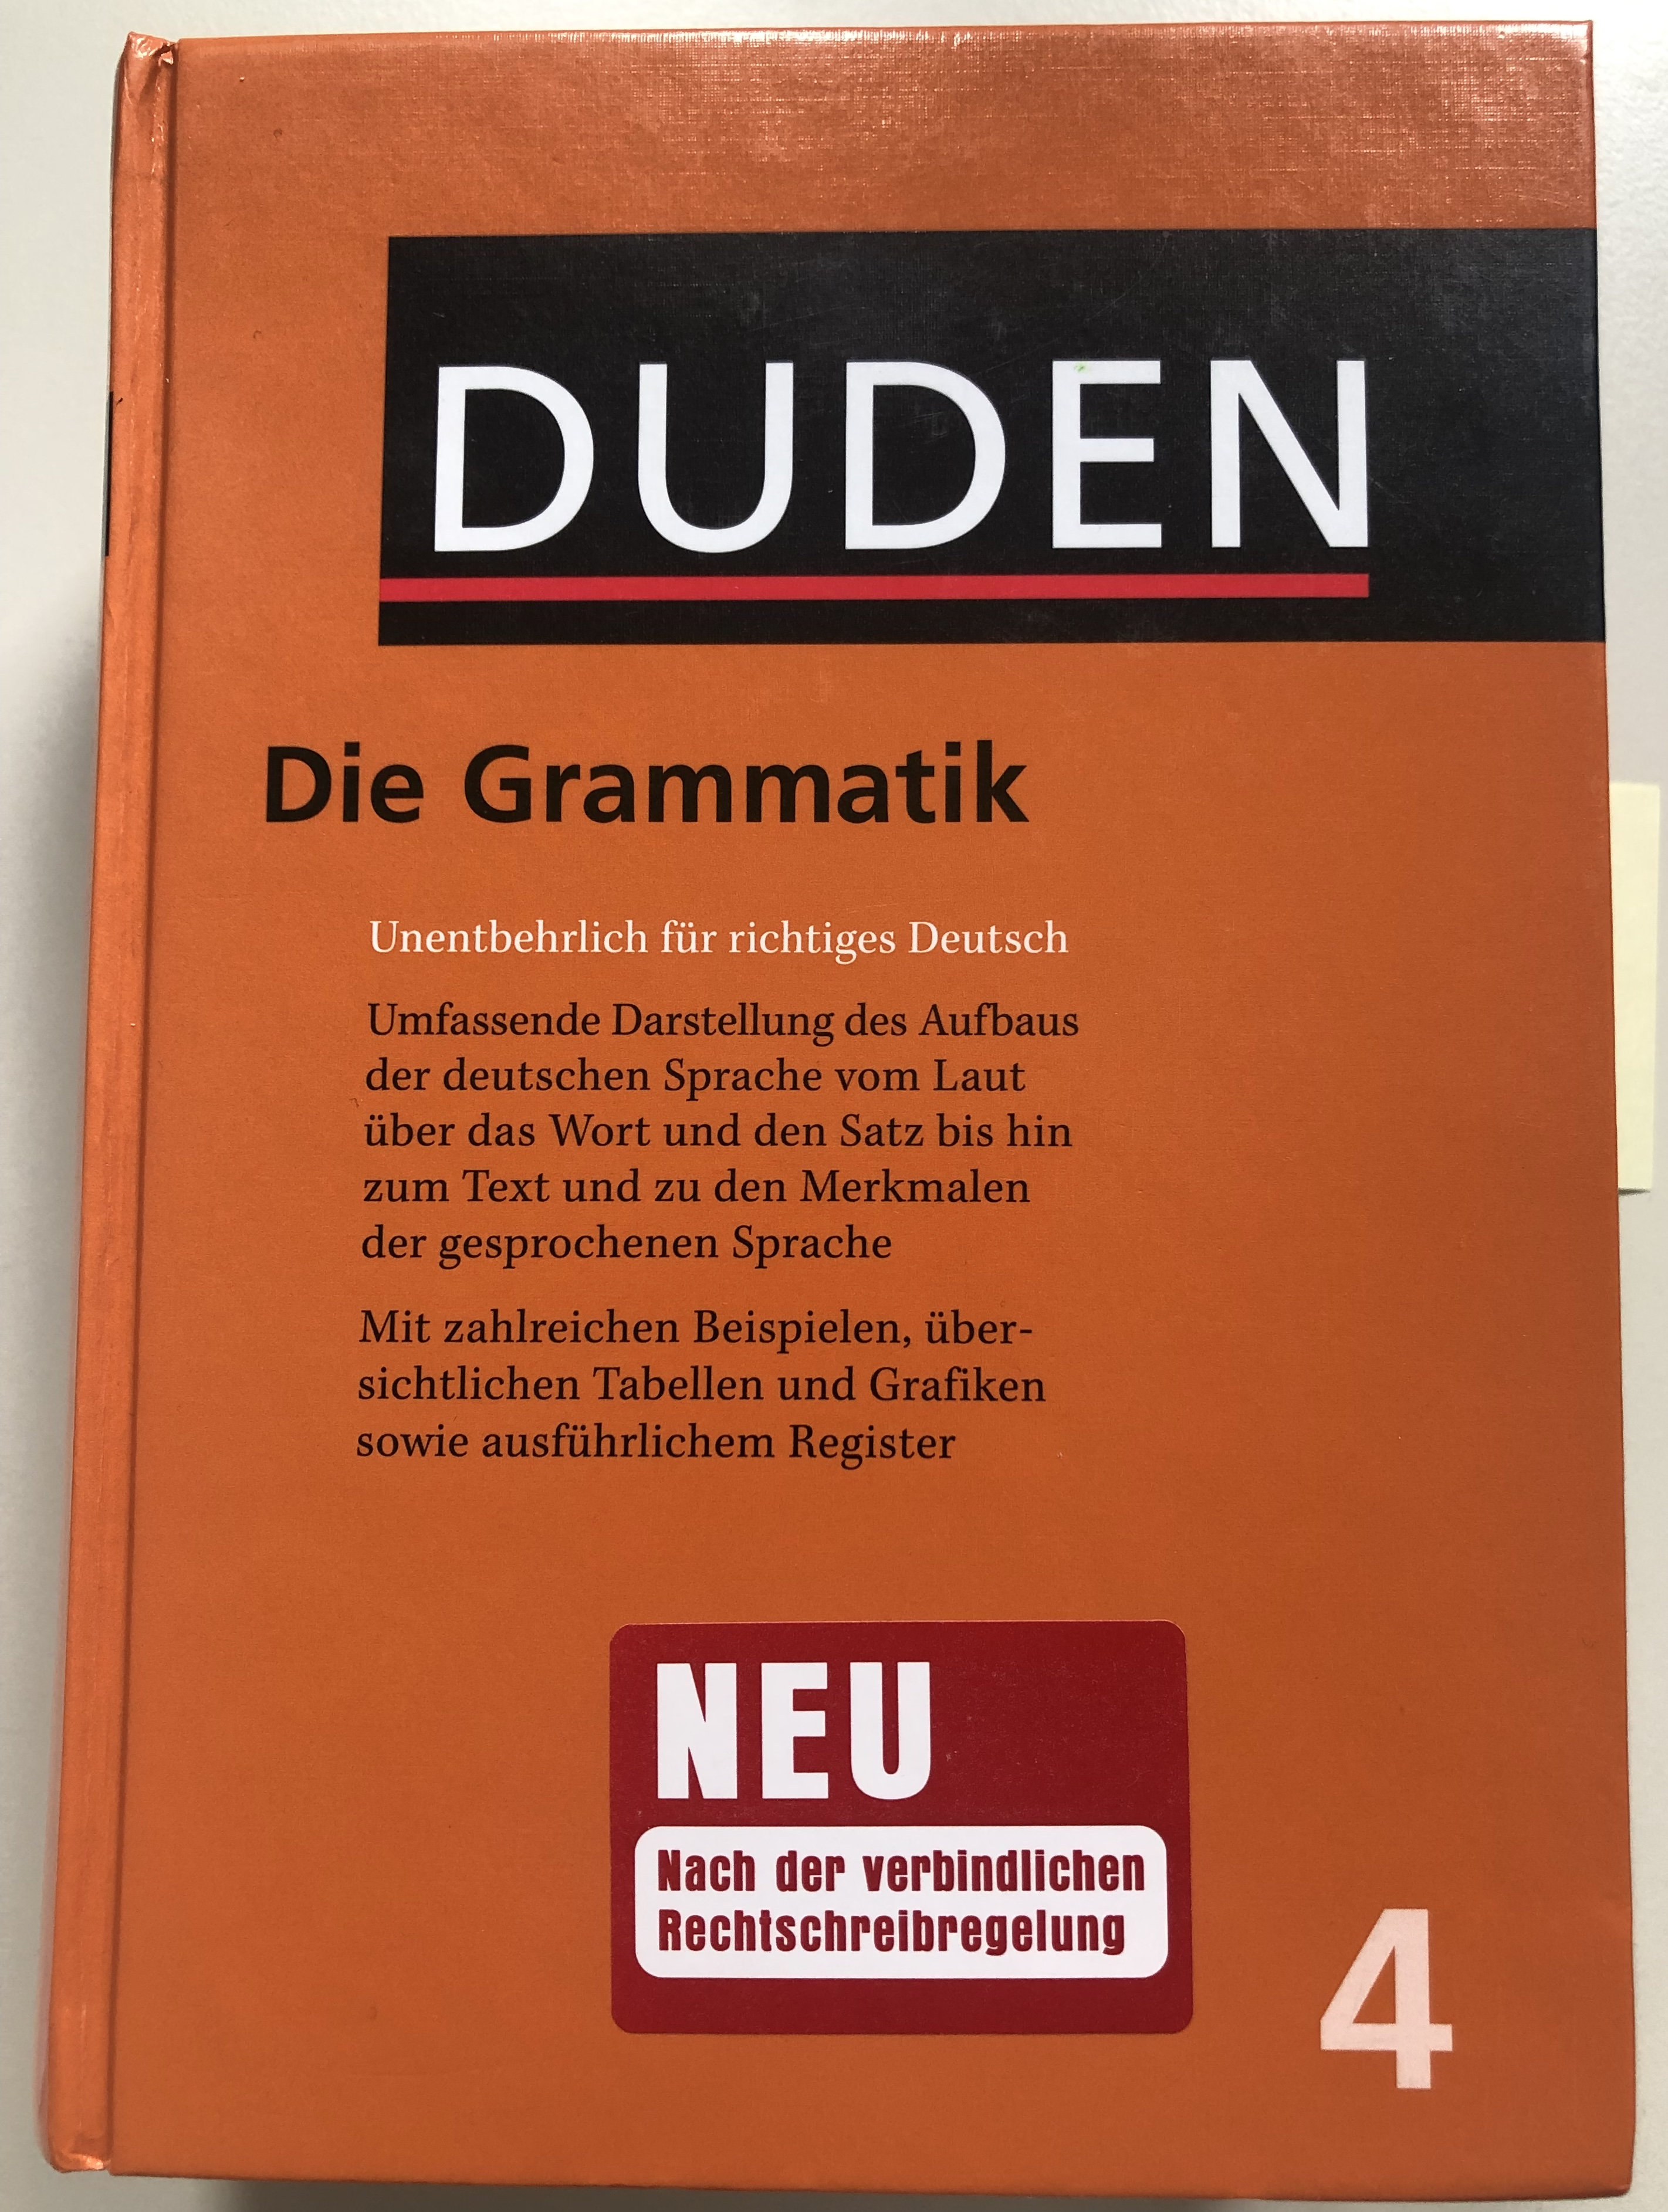
\includegraphics[width=.45\textwidth]{material/DudenRichtigesDeutsch}

\end{frame}


%%%%%%%%%%%%%%%%%%%%%%%%%%%%%%%%%%%
\begin{frame}

\begin{itemize}
	\item<1-> Grammatik als \textbf{Lehrbuch} oder \textbf{Nachschlagewerk}
	\item[]
	\item<2-> Grammatik für den Fremdsprachenunterricht (\zB \citealp{Helbig&Buscha05a})
	\item[]
	\item<3-> Grammatik als \textbf{Sprachtheorie} \citep[vgl.][]{MuellerGT-Eng2}, \zB Generative Grammatik (GG) (vgl. \citealp{Philippi&Tewes10a}) oder Dependenzgrammatik (vgl. \citealp{Agel00a})
	\item[]
	\item<4-> In diesem Seminar verstehen wir \textbf{Grammatik} als:

	\begin{itemize}
		\item<4-> \textbf{System}, das Laute und Bedeutungen regelhaft einander zuordnet und das gesamte Regelsystem einer Sprache umfasst.
		\item<4-> Wir befassen uns mit Grammatik mit einer \textbf{deskriptiven} Methodik
                  (d.\,h. nicht präskriptiv) und verwenden dafür (bzw.\ bilden dadurch)
                  \textbf{Grammatiktheorien} (z.\,B. GG).
	\end{itemize}

\end{itemize}

\end{frame}


%%%%%%%%%%%%%%%%%%%%%%%%%%%%%%%%%%%
%%%%%%%%%%%%%%%%%%%%%%%%%%%%%%%%%%%
\subsection{Modularität der Grammatik}

%% MyP: Contents
\iftoggle{sectoc}{
\frame{
%\begin{multicols}{2}
\frametitle{~}
	\tableofcontents[currentsubsection, subsubsectionstyle=hide]
%\end{multicols}
}
}

%% StM: Contents
\iftoggle{gliederung}{
	
	\outline{
		\begin{itemize}
			
			\item Grammatik
			\item Grammatikbegriff
			\item \blaubf{Modularität der Grammatik}
			%% Lexikon
			%% Phonologische Komponente
			%% Morphologische Komponente
			%% Syntaktische Komponente
			%% Semantische Komponente
			%% Architektur des Sprachsystems
			\item Linguistische Teildisziplinen
			\item Linguistik als Geistes- und/oder Naturwissenschaft
			\item Sprachwissenschaft \vs Linguistik
			
		\end{itemize}
	}
}
%%%%%%%%%%%%%%%%%%%%%%%%%%%%%%%%%%%

\begin{frame}{Modularität der Grammatik}
	
\begin{itemize}
	\item hauptsächlich in der Generativen Grammatik angenommen\\
              (in anderen Grammatiktheorietraditionen umstritten)
	\medskip
	\item Sprachvermögen $\rightarrow$ modular organisiert
	\medskip
	\item<2-> Grammatik (oder Sprache) ist ein \textbf{Modul} im \textbf{menschlichen kognitiven System}.
	\item<2-> Dieses (Sprach)modul besteht zugleich aus \textbf{miteinander interagierenden Teilmodulen} (auch sprachlichen Teilmodulen, grammatischen Ebenen oder sprachlichen Komponenten).
	\medskip
	\item<3-> Wie \textbf{selbstständig} diese Module sind, ist umstritten.
	\medskip
	\item<3-> Die \textbf{Evidenz} für eine Modularisierung findet die GG in der Aphasie-, Versprecher- und Spracherwerbsforschung.  
\end{itemize}

\end{frame}


%%%%%%%%%%%%%%%%%%%%%%%%%%%%%%%%%%%
\begin{frame}
\frametitle{Module}
\begin{itemize}
	\item Folgende Module werden angenommen (vgl. \citealp{Abramowski2016}):
		
	\begin{itemize}
%		\item[]
		\item Lexikon
%		\item[]
		\item Phonologische Komponente
%		\item[]
		\item Morphologische Komponente
%		\item[]
		\item Syntaktische Komponente
%		\item[]
		\item Semantische Komponente
%		\item[]
	\end{itemize}
		
	\item<2-> Jedes sprachliche Modul besteht zugleich aus:
	
	\begin{enumerate}
		\item<2-> einem Inventar von komponentenspezifisch kategorisierten \textbf{Minimaleinheiten}\\
                         (\zB Morphem in der Morphologie) und
		\item<2-> einer Menge von komponentenspezifischen \textbf{Regeln zur Kombination} dieser Minimaleinheiten zu wohlgeformten komplexen Einheiten. 
	\end{enumerate}		  
		
\end{itemize}

\end{frame}


%%%%%%%%%%%%%%%%%%%%%%%%%%%%%%%%%%%
%%%%%%%%%%%%%%%%%%%%%%%%%%%%%%%%%%%
\subsubsection{Lexikon}
%%% MyP: Contents
%\iftoggle{sectoc}{
%	\frame{
%		%\begin{multicols}{2}
%		\frametitle{~}
%		\tableofcontents[currentsubsubsection]
%		%\end{multicols}
%	}
%}
%%%%%%%%%%%%%%%%%%%%%%%%%%%%%%%%%%%

\begin{frame}{Lexikon}
	
	\begin{itemize}
		\item \textbf{Repräsentation von Wörtern} und Wortteilen einer Sprache mit der \textbf{Information} über deren:

		\begin{enumerate}
			\item[]
			\item Aussprache (phonologische Information)
			\item[]
			\item interne Struktur (morphologische Information)
			\item[]
			\item syntaktische Kategorie und syntaktisches Kombinationspotential (syntaktische Information)
			\item[]
			\item Bedeutung (semantische Information) 
			\item[]
			\item idiosynkratische Information (nicht ableitbare Information)
		\end{enumerate}		  
			
	\end{itemize}
		
\end{frame}


%%%%%%%%%%%%%%%%%%%%%%%%%%%%%%%%%%%
\begin{frame}{Lexikon}
			
\begin{itemize}
	\item Eintrag für den Verbstamm \emph{geb-} (von \emph{geben}): \ab{\textsc{geb-}}

	\begin{enumerate}
		\item[]
		\item Phonologische Information: \textipa{/ge\textlengthmark{}b/}
		\item[]
		\item Morphologische Information: [\textsubscript{V-Stamm}\ab{geb-}] 
		\item[]
		\item Syntaktische Information (ditransitives Verb):\\
			NP\textsubscript{\alertred{1}\{\textsc{nom}\}}$+$
			NP\textsubscript{\alertred{2}\{\textsc{dat}\}}$+$
			NP\textsubscript{\alertred{3}\{\textsc{akk}\}}$+$
			V
					
		\item[]
		\item Semantische Information (Verb des Besitzwechsels):\\
			NP\textsubscript{\alertred{1}\{\textsc{agens}\}}$+$
			NP\textsubscript{\alertred{2}\{\textsc{goal}\}}$+$
			NP\textsubscript{\alertred{3}\{\textsc{thema}\}}$+$
			V \\
			$\approx$
			\gq{NP\textsubscript{\alertred{1}} macht, dass NP\textsubscript{\alertred{2}} NP\textsubscript{\alertred{3}} erhält.} 
	\end{enumerate}		  


\ea (\dots dass) Luise\MyPdown{\alertred{1}} Jacob\MyPdown{\alertred{2}} das Buch\MyPdown{\alertred{3}} gibt
\z 
\end{itemize}

\end{frame}


%%%%%%%%%%%%%%%%%%%%%%%%%%%%%%%%%%%
%%%%%%%%%%%%%%%%%%%%%%%%%%%%%%%%%%%
\subsubsection{Phonologische Komponente}
%%% MyP: Contents
%\iftoggle{sectoc}{
%	\frame{
%		%\begin{multicols}{2}
%		\frametitle{~}
%		\tableofcontents[currentsubsubsection]
%		%\end{multicols}
%	}
%}
%%%%%%%%%%%%%%%%%%%%%%%%%%%%%%%%%%%

\begin{frame}{Phonologische Komponente}

	\begin{itemize}
		\item Sie beschränkt das \textbf{Lautinventar} einer Sprache.
		\item[]
		\item Sie regelt die \textbf{Lautkombinatorik} und \textbf{-veränderung}.
		\item[]
		\item Festlegung von \textbf{Wort-} und \textbf{Satzakzent}:
		
\pause
		 \begin{itemize} 
                 \item Wieso spricht man \ab{Hund} mit \textipa{[t]} aber \ab{Hunde} mit \textipa{[d]} aus?
\pause
                 \item Kann ein Wort im Deutschen mit der Lautfolge \textipa{[Ng]} beginnen?
\pause
	         \item Was ist der Unterschied zwischen \abu{HAUStürgriff} und \abu{HausTÜRgriff}?
		\end{itemize}	  
	
	\end{itemize}
	
\end{frame}


%%%%%%%%%%%%%%%%%%%%%%%%%%%%%%%%%%%
%%%%%%%%%%%%%%%%%%%%%%%%%%%%%%%%%%%
\subsubsection{Morphologische Komponente}
%%% MyP: Contents
%\iftoggle{sectoc}{
%	\frame{
%		%\begin{multicols}{2}
%		\frametitle{~}
%		\tableofcontents[currentsubsubsection]
%		%\end{multicols}
%	}
%}
%%%%%%%%%%%%%%%%%%%%%%%%%%%%%%%%%%%

\begin{frame}{Morphologische Komponente}

\begin{itemize}
	\item Sie regelt die \textbf{interne Struktur von Wörtern}.
	\item[]
	\item Bildung von neuen Wörtern und Wortformen
\pause
				
\ea Wie hängen \ab{kaufen} und \ab{kaufbar} zusammen?
\pause
	\ex Was zeigt \ab{-st} bei der Bildung neuer Verbformen an?
\z
			
\end{itemize}

\end{frame}


%%%%%%%%%%%%%%%%%%%%%%%%%%%%%%%%%%%
\begin{frame}{Morphologische Komponente}

	\ea Warum ist die eine Struktur des Wortes \ab{Bedeutungsableitung} intuitiv nicht korrekt und die andere schon?
	\z
			

\begin{columns}

\column[b]{.4\linewidth}		
\begin{figure}[b]
	
\scriptsize{
		\begin{forest}MyP edges
		[Bedeutungsableitung [Be][deutungsableitung [deut][ungsableitung [ungsableit [ung][sableit [sab [s][ab]][leit]]][ung]]]]
		\end{forest}
}
		
\caption{Ungrammatisch}

\end{figure}

\column[b]{.4\linewidth}
\begin{figure}[b]
	\scriptsize{
		\begin{forest}MyP edges
		[Bedeutungsableitung [Bedeutungs [Bedeutung [Bedeut [Be][deut]][ung]][s]][ableitung [ableit [ab][leit]][ung]]]
		\end{forest}}
			
	\caption{Grammatisch}

\end{figure}

\end{columns}
\end{frame}


%%%%%%%%%%%%%%%%%%%%%%%%%%%%%%%%%%%
%%%%%%%%%%%%%%%%%%%%%%%%%%%%%%%%%%%
\subsubsection{Syntaktische Komponente}
%%% MyP: Contents
%\iftoggle{sectoc}{
%	\frame{
%		%\begin{multicols}{2}
%		\frametitle{~}
%		\tableofcontents[currentsubsubsection]
%		%\end{multicols}
%	}
%}
%%%%%%%%%%%%%%%%%%%%%%%%%%%%%%%%%%%
	
\begin{frame}{Syntaktische Komponente}

\begin{itemize}
	\item Sie regelt die \textbf{Struktur} von \textbf{Phrasen und Sätzen}.

	\ea Wieso ist die Phrase (\ref{ex1a}) grammatisch und die Phrase (\ref{ex1b}) nicht?
	\ea[ ]{die Königin von Schweden aus Deutschland}\label{ex1a}
	\ex[*]{die Königin aus Deutschland von Schweden}\label{ex1b}
	\z
	\z

	\ea Warum ist ein Satz wie (\ref{ex2a}) ungrammatisch (trotz alphabetischer Anordnung der Wörter), während (\ref{ex2b}) grammatisch ist?
	\ea[*]{Buch Chomsky das ich kaufen morgen von werde.}\label{ex2a}
	\ex[]{Das Buch von Chomsky werde ich morgen kaufen.}\label{ex2b}
	\z \z
	
	\ea Aus welchem Grund hat der Satz unter (\ref{ex3}) zwei Bedeutungen? 
	\ea Maria hat Peter gesehen.\label{ex3}
\z \z
			
\end{itemize}

\end{frame}


%%%%%%%%%%%%%%%%%%%%%%%%%%%%%%%%%%%
%%%%%%%%%%%%%%%%%%%%%%%%%%%%%%%%%%%
\subsubsection{Semantische Komponente}
%%% MyP: Contents
%\iftoggle{sectoc}{
%	\frame{
%		%\begin{multicols}{2}
%		\frametitle{~}
%		\tableofcontents[currentsubsubsection]
%		%\end{multicols}
%	}
%}
%%%%%%%%%%%%%%%%%%%%%%%%%%%%%%%%%%%
		
\begin{frame}{Semantische Komponente}
	
	\begin{itemize}
		\item Semantische Komponente regelt die \textbf{Bedeutungsherleitung} komplexerer Einheiten (komplexer Wörter, Phrasen und Sätze).
%		\item[]
		\item<2-> Wichtig bei der Herleitung $\rightarrow$ \textbf{Bedeutung der Bestandteile + Bedeutung der Struktur} (Kompositionalitäts- oder \textbf{Fregeprinzip})
				
\ea Worin besteht der Bedeutungsunterschied zwischen den Verben \ab{arbeiten} und \ab{bearbeiten}?
	\ex Wieso haben die Sätze (\ref{ex4a}) und (\ref{ex4b}) nicht die gleiche Bedeutung, obwohl sie aus den gleichen Wörtern bestehen?
	
		\ea maria hat peter gesehen \label{ex4a}
			\ex hat maria peter gesehen \label{ex4b}
		\z 

	\ex Warum bedeutet \ab{sich} in (\ref{ex5a}) und (\ref{ex5b}) nicht dasselbe?

		\ea Maria verspricht \textbf{sich}, Mario zu treffen. \label{ex5a}
			\ex Maria verspricht Mario, \textbf{sich} zu treffen. \label{ex5b}
		\z

\z
	\end{itemize}
	
\end{frame}


%%%%%%%%%%%%%%%%%%%%%%%%%%%%%%%%%%%
%%%%%%%%%%%%%%%%%%%%%%%%%%%%%%%%%%%
\subsubsection{Architektur des Sprachsystems}
%%% MyP: Contents
%\iftoggle{sectoc}{
%	\frame{
%		%\begin{multicols}{2}
%		\frametitle{~}
%		\tableofcontents[currentsubsubsection]
%		%\end{multicols}
%	}
%}
%%%%%%%%%%%%%%%%%%%%%%%%%%%%%%%%%%%
		
\begin{frame}{Architektur des Sprachsystems}
	
	\begin{itemize}
		\item Sprachliche Strukturbildung wird durch bereits erwähnte Komponenten geregelt.
		\item[]
		\item<2-> Außerdem interagiert das grammatische System der Sprache mit den folgenden \textbf{außersprachlichen Ebenen}:
				
		\begin{itemize}
			\item[]
			\item<3-> dem \textbf{artikulatorisch-perzeptorischen Apparat}\par
				(den biologischen Gegebenheiten zur Produktion und Rezeption von Sprachlauten)
			\item[]
			\item<3->[] und
			\item[]
			\item<4-> dem \textbf{konzeptuell-intentionalen System}, d.\,h. dem Bereich der Kognition, der sich mit Bedeutung befasst.\par
				Das konzeptuell-intentionale System wird wiederum durch Weltwissen, Kontextwissen und analytisches Wissen gespeist.
		\end{itemize}
			
	\end{itemize}
		
\end{frame}


%%%%%%%%%%%%%%%%%%%%%%%%%%%%%%%%%%%
%\begin{frame}{Architektur des Sprachsystems}

%\begin{figure}[H]
%\centering
				
%	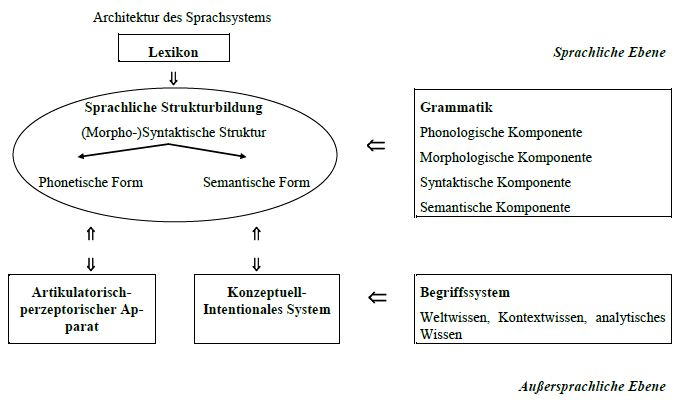
\includegraphics[width=\textwidth]{material/03ArchitekturSprachsystem.jpg}
%	\caption{Architektur des Sprachsystems \citep{Abramowski2016}}
%	\label{Zeichen3}

%\end{figure}

%\end{frame}			


%%%%%%%%%%%%%%%%%%%%%%%%%%%%%%%%%%%
\begin{frame}

\begin{figure}
\centering
\small
\begin{minipage}{0.55\textwidth}
\centering
\fbox{Lexikon}\\
\Large
$ \Downarrow $
\end{minipage}
%
\begin{minipage}{0.1\textwidth}
\centering
\hfill
\end{minipage}
%
\begin{minipage}[t]{0.3\textwidth}
\centering
\textit{Sprachliche Ebene}
\end{minipage}

\begin{minipage}[t]{0.55\textwidth}
\centering
\outputbox{\centering Sprachliche Strukturbildung\\
\begin{forest}sm edges,
[(morpho-)syntaktische Struktur
[Phonetische Form]
[Semantische Form]
]
\end{forest}}
\begin{tabular}{cp{3cm}c}
\Large
$ \Updownarrow $ && \Large $ \Updownarrow $\\
\end{tabular}
\end{minipage}
%
\begin{minipage}[c]{0.1\textwidth}
\centering
\Large
$ \Leftarrow $
\end{minipage}
%
\begin{minipage}[t]{0.3\textwidth}
\centering
\small
\outputbox{
Grammatik
\begin{itemize*}
\item Phonologische Komponente\\
\item Morphologische K.\\
\item Syntaktische K.\\
\item Semantische K.
\end{itemize*}}
\end{minipage}

\begin{minipage}{0.24\textwidth}
\centering
\outputbox{\centering Artikulatorisch-perzeptorischer Apparat}
\end{minipage}
%
\begin{minipage}[c]{0.05\textwidth}
\hfill
\end{minipage}
%
\begin{minipage}{0.24\textwidth}
\centering
\outputbox{\centering Konzeptuell-Intentionales System}
\end{minipage}
%
\begin{minipage}{0.1\textwidth}
\centering
\Large
$\Leftarrow$
\end{minipage}
%
\begin{minipage}{0.3\textwidth}
\outputbox{Begriffssystem
\newline
\small
\raggedright
Weltwissen, Kontextwissen, analytisches Wissen}
\end{minipage}

\begin{minipage}{0.65\textwidth}
\hfill
\end{minipage}
%
\begin{minipage}{0.3\textwidth}
\centering
\small
\textit{Außersprachliche Ebene}
\end{minipage}
\caption{Die Architektur des Sprachsystems \citep[vgl.][]{Abramowski2016}}
\end{figure}

\end{frame}


%%%%%%%%%%%%%%%%%%%%%%%%%%%%%%%%%%%
%%%%%%%%%%%%%%%%%%%%%%%%%%%%%%%%%%%
\subsection{Linguistische Teildisziplinen}		

%% MyP: Contents
\iftoggle{sectoc}{
\frame{
%\begin{multicols}{2}
	\tableofcontents[currentsubsection, subsubsectionstyle=hide]
%\end{multicols}
}
}

%% StM: Contents
\iftoggle{gliederung}{
	
	\outline{
		\begin{itemize}
			
			\item Grammatik
			\item Grammatikbegriff
			\item Modularität der Grammatik
			%% Lexikon
			%% Phonologische Komponente
			%% Morphologische Komponente
			%% Syntaktische Komponente
			%% Semantische Komponente
			%% Architektur des Sprachsystems
			\item \blaubf{Linguistische Teildisziplinen}
			\item Linguistik als Geistes- und/oder Naturwissenschaft
			\item Sprachwissenschaft \vs Linguistik
			
		\end{itemize}
	}
}
%%%%%%%%%%%%%%%%%%%%%%%%%%%%%%%%%%%

\begin{frame}{Linguistische Teildisziplinen}

	\begin{tabular}{ll}
\multirow{4}{*}{im engeren Sinne (System):} & Phonologie \\
																	& Morphologie \\
																	& Syntax \\
																	& Semantik \\
\hline
\multirow{3}{*}{im weiteren Sinne (Gebrauch):} & Phonetik \\
																		& Graphematik \\
																		& Pragmatik \\
\hline
\multirow{5}{*}{Linguistische Methoden:} & Psycholinguistik \\
& Soziolinguistik \\
& Historische Linguistik \\
& Korpuslinguistik \\
& \dots \\
	\end{tabular}
	
\end{frame}



%%%%%%%%%%%%%%%%%%%%%%%%%%%%%%%%%%%
%%%%%%%%%%%%%%%%%%%%%%%%%%%%%%%%%%%
\subsection{Linguistik als Geistes- und/oder Naturwissenschaft}		

%% MyP:Contents
\iftoggle{sectoc}{
\frame{
%\begin{multicols}{2}
	\tableofcontents[currentsubsection, subsubsectionstyle=hide]
%\end{multicols}
}
}

%% StM: Contents
\iftoggle{gliederung}{
	
	\outline{
		\begin{itemize}
			
			\item Grammatik
			\item Grammatikbegriff
			\item Modularität der Grammatik
			%% Lexikon
			%% Phonologische Komponente
			%% Morphologische Komponente
			%% Syntaktische Komponente
			%% Semantische Komponente
			%% Architektur des Sprachsystems
			\item Linguistische Teildisziplinen
			\item \blaubf{Linguistik als Geistes- und/oder Naturwissenschaft}
			\item Sprachwissenschaft \vs Linguistik
			
		\end{itemize}
	}
}
%%%%%%%%%%%%%%%%%%%%%%%%%%%%%%%%%%%

\begin{frame}{Linguistik als Geistes- und/oder Naturwissenschaft}

	\begin{itemize}
		\item \textbf{Geisteswissenschaft}
		
		\begin{itemize}
			\item Verstehen von individuellen Leistungen des Geistes\par
				(eines Menschen, einer Gemeinschaft, einer Epoche)
			\item Verstehen von kulturellen Beziehungen und Entwicklungen
			\item[$\rightarrow$] Methode: \textbf{Hermeneutik} (Annähern durch Verstehen)
		\end{itemize}
		
		\item[]
		\item \textbf{Naturwissenschaft}
		
		\begin{itemize}
			\item Erklärung von naturgesetzlichen Kausalitäten und Zusammenhängen
			\item[$\rightarrow$] Methode: \textbf{Experiment}
		\end{itemize}
		
	\end{itemize}
	
\end{frame}		


%%%%%%%%%%%%%%%%%%%%%%%%%%%%%%%%%%%
\begin{frame}
\frametitle{Linguistik als Naturwissenschaft}

	\begin{itemize}
		\item Linguistik \textit{eher} naturwissenschaftlich ausgerichtet\par
			(im Gegensatz zur Literaturwissenschaft)
		
		\begin{itemize}
			\item[]
			\item \textbf{Beobachtung} und \textbf{Analyse} von Gesetzen natürlicher Sprachen mit dem Ziel ihre \textbf{Systematik} aufzudecken (\zB Syntax)
			\item[]
			\item<2-> Arbeit mit \textbf{empirischen} Verfahren wie Experimenten (\zB Psycholinguistik) oder wie Ansammlungen von Daten (\zB Korpuslinguistik) als Evidenz $\rightarrow$ \textbf{Naturwissenschaft}
			\item[]
			\item<3-> Beschäftigung mit der \textbf{Geschichte} einer Sprache (\zB Historische Linguistik) und mit den \textbf{sozialen} und kulturellen Bedingungen vom Sprachwandel (\zB Soziolinguistik) $\rightarrow$ \textbf{Geisteswissenschaft}
			\item[]
			\item<4-> Untersuchung des vielleicht \textbf{zentralsten Outputs des Geistes}:\par
				der Sprache (vgl. \citealt{Meibauer&Co07a})
		\end{itemize}
		
	\end{itemize}
	
\end{frame}		


%%%%%%%%%%%%%%%%%%%%%%%%%%%%%%%%%%%
%%%%%%%%%%%%%%%%%%%%%%%%%%%%%%%%%%%
\subsection{Sprachwissenschaft \vs Linguistik}

%% MyP: Contents
\iftoggle{sectoc}{
\frame{
%\begin{multicols}{2}
	\tableofcontents[currentsubsection, subsubsectionstyle=hide]
%\end{multicols}
}
}

%% StM: Contents
\iftoggle{gliederung}{
	
	\outline{
		\begin{itemize}
			
			\item Grammatik
			\item Grammatikbegriff
			\item Modularität der Grammatik
			%% Lexikon
			%% Phonologische Komponente
			%% Morphologische Komponente
			%% Syntaktische Komponente
			%% Semantische Komponente
			%% Architektur des Sprachsystems
			\item Linguistische Teildisziplinen
			\item Linguistik als Geistes- und/oder Naturwissenschaft
			\item \blaubf{Sprachwissenschaft \vs Linguistik}
			
		\end{itemize}
	}
}
%%%%%%%%%%%%%%%%%%%%%%%%%%%%%%%%%%%

\begin{frame}{Sprachwissenschaft \vs Linguistik}

	\begin{itemize}
		\item<1-> Linguistik und Sprachwissenschaft werden \idR \textbf{synonymisch} gebraucht.
%		\item[]
		\item<2-> Unterscheidung:
		
		\begin{itemize}
%			\item[]
			\item<2-> Linguistik als \textbf{Teildisziplin} der Sprachwissenschaft
			\item<3-> \gqq{\textbf{Innere Sprachwissenschaft}} $\approx$ Linguistik $\rightarrow$ Beschäftigung mit innersprachlichen Sachverhalten und Entwicklungen (Sprache als System)
			\item<4-> \gqq{\textbf{Äußere Sprachwissenschaft}} $\rightarrow$ Beschäftigung mit kulturellen, sozialen, ökonomischen, politischen, usw. Bedingungen der Existenz und der Geschichte von Sprache, d.\,h. den äußeren (auch \textit{außersprachlich} genannten) Faktoren (vgl. \citealp{Glueck05a})
		\end{itemize}
		
%		\item[]
		\item<5-> In diesem Kurs werden wir jedoch beide Begriffe gleichbedeutend verwenden.
	\end{itemize}
	
\end{frame}

%%%%%%%%%%%%%%%%%%%%%%%%%%%%%%%%%%%

\begin{frame}{Abbildungen}
	\begin{itemize}
		\item ABBILDUNG -- Machicao y Priemer, Antonio: \gqq{Duden} (Privatfoto).
	\end{itemize}
\end{frame}


